% Když budete cokoli psát: ukládejte starší verze vždy odděleně, abyste se 
% k nim mohli kdykoli vrátit. Kusy textu, které jste se rozhodli nepoužít, taky ukládejte do zvláštního souboru. Smazat se to dá vždycky, ale psát to znova je opruz. 

% A POŘÁD ZÁLOHUJTE. POŘÁD !!!

\documentclass[12pt, a4paper, oneside]{article} 
% velikost písma, stránky, typ dokumentu -- detaily viz literatura

\usepackage{czech} % nastavení češtiny
%\usepackage[latin2]{inputenc}
%\usepackage[cp1250]{inputenc} % pro win1250
\usepackage[utf8]{inputenc}
\usepackage{wrapfig} % nastavení obtékání textu
\usepackage{graphicx,amsmath} % nastavení grafiky, matematiky
\usepackage{subfig} % více obrázků vedle sebe 
\usepackage{float}

\usepackage{tocloft} %přidá tečky do obsahu ke kapitolám /sekcím 
\renewcommand{\cftsecdotsep}{\cftdotsep}

\usepackage[bookmarksopen,colorlinks,plainpages=false,linkcolor=black,urlcolor=blue,citecolor=black,filecolor=black,menucolor=black,unicode=true]{hyperref}
%bookmarksopen -- open up bookmark tree 
%colorlinks -- zbarví odkazy (implicitně orámovaný nezbarvený text)
%urlcolor -- barva odkazů (implicitně magenta) 
%linkcolor=black -- barva odkazů v obsahu (implicitně red)


% \usepackage{parskip} -- zapne americké odstavce v celé práci

\addtolength{\textwidth}{-2mm} 
\addtolength{\hoffset}{4mm}  % posun textu kvůli kroužkové vazbě  

\setlength{\intextsep}{5mm} % nastavení mezery okolo obrázků

% nastavení příkazu >\figcaption pro popis čehokoli, jako by to byly obrázky 
\makeatletter   
\newcommand\figcaption{\def\@captype{figure}\caption}
\makeatother

\def\refname{Literatura} 
% přejmenuje anglický název Reference na české Literatura


%\makeindex % příprava pro výrobu indexu (jestli ho chcete)

%%    VLNKA <fileinput>  KkSsVvZzOoUuAaIi        
% Defaultni  koncovka pro <fileinput> je  ".tex"
%FIXME: haze error
%\cstieon % Vypne chovani vlnky jako tvrde mezery v matematickem rezimu

%%%%%%%%%%%%%%%%%%%%%%%%%%%%%%%%%%%%%%%%%%%%%%%%%%%%%%%%%%%%%%%
%V PROSTŘEDÍ ROVNIC SE NESMÍ VYSKYTOVAT PRÁZDNÝ ŘÁDEK
%
%PROGRAMY VLNKA A CSINDEX SE MUSÍ SPUSTIT SAMOSTATNĚ
%%%%%%%%%%%%%%%%%%%%%%%%%%%%%%%%%%%%%%%%%%%%%%%%%%%%%%%%%%%%%%%

% definice příkazů 
\newcommand{\D}{\medskip \noindent} % nový odstavec v "americkém" formátování 
\newcommand{\B}{\textbf} %tučné písmo
\newcommand{\A}{\mathbf} %tučné písmo v matematickém režimu
\newcommand{\TO}{\ensuremath{\boldsymbol\Omega}} % tučný znak velké omega -- pro ohmy
\newcommand{\I}{\index}  % vytváří položku indexu (asi nepoužijete)
\newcommand{\Deg}[1][]{\ensuremath{{#1}^\circ}} % vysází značku stupně Celsia
\newcommand{\Def}{\footnotesize Definice: \normalsize}
\newcommand{\Pos}{\footnotesize Experiment: \normalsize}
\newcommand{\Odv}{\footnotesize Odvození: \normalsize}
\newcommand{\Vym}{\footnotesize Vymezení pojmu: \normalsize}
\newcommand{\Ob}{obrázek }
\newcommand{\It}{\textit}  % kurzíva
\newcommand{\M}{\mathrm}   % v prostředí rovnic nastaví normální písmo (místo kurzívy ) 
\newcommand{\F}{\footnotesize} % zmenšená velikost písma
\newcommand{\N}{\normalsize} % normální velikost písma
%\newcommand{\U}{\underline}  % podtržené písmo
\newcommand{\e}{\ensuremath} 
% další příkaz se aplikuje, pouze, když jste v matematickém režimu

%\hyphenation{Pusť-me pla-tí hod-no-ty do-sa-dí-me za-da-né}
% dělení slov, kdyby implicitní nevyhovovalo

\linespread{1.3} 
% řádkování 1,5x  
% použijete podle situace  

\unitlength=1mm % nastavení volby jednotek 

% konec hlavičky
%%%%%%%%%%%%%%%%%%%%%%%%%%%%%%%%%%%%%%%%%%%%%%%%%%%%%%%%%%%%%%%%%%%
%%%%%%%%%%%%%%%%%%%%%%%%%%%%%%%%%%%%%%%%%%%%%%%%%%%%%%%%%%%%%%%%%%%

\begin{document} % začátek textové části 

% titulní strana
\pagestyle{empty} % vynechá číslování
 
\voffset = -20mm % posun začátku textu výš
\enlargethispage{60mm} % zvětší oblast tisku pro tuto stránku   

\begin{center}
 
\Large \B{STŘEDOŠKOLSKÁ ODBORNÁ ČINNOST}

\vspace{60mm}

\huge %\LARGE
\B{GRAFICKÉ UŽIVATELSKÉ ROZHRANÍ} 
% na titulní straně může být stručnější, pokud je to potřeba  

\Large

\vspace{90mm}


\B{Vojtěch Boček} \\

\vspace{40mm}

\B{Brno 2012}


\end{center}

\newpage % konec titulní strany 
%%%%%%%%%%%%%%%%%%%%%%%%%%%%%%%%%%%%%%%%%%%%%%%%%%%%%%%%%%%%%%%%%%%%%%%%%%%

% vnitřní titulní strana
\voffset = -20mm % posun začátku textu výš
\enlargethispage{60mm} % zvětší oblast tisku pro tuto stránku   

\begin{center}

\Large \B{STŘEDOŠKOLSKÁ ODBORNÁ ČINNOST}  \\
\vspace{10mm}
 \normalsize 
\B{Obor SOČ: 18. Informatika}% číslo a název -- vyplníme spolu 

\vspace{45mm}

\LARGE %\huge 
\B{GRAFICKÉ UŽIVATELSKÉ ROZHRANÍ} 
\end{center}  
\large

\vspace{50mm}


\begin{tabbing}
\hspace{10mm} \= \hspace{30mm}  \=   \kill % nastavení zarážek 
  \> \B{Autor:}  \> \B{Vojtěch Boček}        \\[8mm] 
  \> \B{Škola:}   \> \B{SPŠ a~VOŠ technická, }     \\
  \>              \> \B{Sokolská 1 602 00 Brno}    \\[8mm]

  \> \B{Konzultant:} \> \B {Jakub Streit} 
\end{tabbing}

\vspace{20mm}

\begin{center}
\B{Brno 2012}

\end{center}
\normalsize
%%%%%%%%%%%%%%%%%%%%%%%%%%%%%%%%%%%%%%%%%%%%%%%%%%%%%%%%%%%%%%%%%%%%%%%%%%%
\newpage  % Prohlášení o autorství  
\voffset = 0mm % posun začátku textu zpět

~ % musí to tu být, aby fungovala svislá mezera

\vspace{10mm}

\section*{Prohlášení}

Prohlašuji, že jsem svou práci vypracoval samostatně, použil jsem pouze 
podklady (literaturu, SW atd.) citované v~práci a~uvedené v~přiloženém seznamu 
a~postup při zpracování práce je v~souladu se zákonem č. 121/2000 Sb., o~právu 
autorském, o~právech souvisejících s~právem autorským a~o~změně některých 
zákonů (autorský zákon) v~platném znění. 
 
\vspace{20mm} 
 
\noindent V~Brně  dne: 6.3.2012 \hspace{50mm}                 podpis:   
 

%%%%%%%%%%%%%%%%%%%%%%%%%%%%%%%%%%%%%%%%%%%%%%%%%%%%%%%%%%%%%%%%%%%%%%%%%%%
\newpage   % Poděkování -- nepovinné 

~ % musí to tu být, aby fungovala svislá mezera

\vspace{120mm}

\section*{Poděkování}

 Děkuji Jakubu Streitovi za rady, obětavou pomoc, velkou trpělivost a~podnětné připomínky poskytované během práce na tomto projektu, a Martinu Vejnárovi za informace o jeho programátoru Shupito.\\% nebo cokoli dle Vašeho uvážení 
 Dále děkuji organizaci DDM Junior, za poskytnutí podpory.\\
 Také bych chtěl poděkovat panu profesorovi Mgr. Miroslavu Burdovi za všeobecnou pomoc s prací.\\
 V neposlední řadě děkuji Martinu Foučkovi za rady a pomoc s Qt Frameworkem.

\D Tato práce byla vypracována za finanční podpory JMK.
 

%%%%%%%%%%%%%%%%%%%%%%%%%%%%%%%%%%%%%%%%%%%%%%%%%%%%%%%%%%%%%%%%%%%%%%%%%%%
\newpage   % Anotace 
~ % musí to tu být, aby fungovala svislá mezera
\vspace{10mm}

\section*{Anotace }

    Cílem této práce bylo vytvořit uživatelské prostředí určené k parsování a~zobrazování surových dat posílaných z mikrokontrolérů v~robotech, digitálních sondách apod. 
Hlavní vlastností programu je modulárnost -- rozdělení na~podčásti určené ke specifickým úkonům (Terminál, grafický parser, vykreslování grafů).

\D \B{Klíčová slova:} parser, analýza dat, program

\section*{Annotation}

    Purpose of this labor is to create graphical user interface for parsing and displaying raw data sent from embedded devices, robots, digital probes and other devices which are using microcontrollers.
Main feature of this application is modularity -- it is divided to sub-sections designed for specific operations (Terminal, graphical parser, graph drawer).

\D \B{Key words:} parser, data analysis, program

\addtolength{\textheight}{30mm} % prodlouží následující stránku

%%%%%%%%%%%%%%%%%%%%%%%%%%%%%%%%%%%%%%%%%%%%%%%%%%%%%%%%%%%%%%%%%%%%%%%%%%%
\newpage

\setlength{\voffset}{-20mm} % posune text/obrázek na této stránce nahoru
%\setcounter{page}{1}  % nastaví čítač stránek znovu od jedné

\tableofcontents  % vysází obsah

\addtolength{\textheight}{-30mm} % zkrátí následující stránku
%%%%%%%%%%%%%%%%%%%%%%%%%%%%%%%%%%%%%%%%%%%%%%%%%%%%%%%%%%%%%%%%%%%%%%%%%%%
\newpage
\setlength{\voffset}{0mm} % posune text/obrázek na této stránce, kam patří
%\pagestyle{headings} % znovu zapne číslování
\pagestyle{plain}
\section*{Úvod}

\addcontentsline{toc}{section}{Úvod} % přidá položku úvod do obsahu
% zde začne text úvodu
%TODO: naší?
Při stavbě robotů (například na soutěž Eurobot) jsem se setkal s problémem  při zpracovávání dat z poměrně velkého množství senzorů, které robot obsahuje, a jejich přehledného zobrazování. Nenašel jsem žádný program, který by mi vyhovoval -- k dispozici jsou pouze komerční aplikace, které stojí poměrně velké množství peněz, anebo aplikace které dokáží zobrazovat pouze v jednom formátu -- typicky graf. Z tohoto důvodu jsem se rozhodl napsat vlastní program.

\section*{Popis rozhraní}
\addcontentsline{toc}{section}{Popis rozhraní}
Svůj program jsem pojmenoval "Lorris", je vytvořený v C++ a využívá Qt Framework(v4.7)\cite{qtfw}, což je multiplatformní framework, který mimo jiné umožňuje spustit aplikaci na více systémech -- testoval jsem na Debian Linux (Wheezy, 64bit) a Windows 7.  

Program je navrhnutý jako modulární aplikace, aby mohl zastřešit několik samostatných částí, které však mají podobnou oblast použití. Základní část programu poskytuje připojení k zařízení (např. robot, deska s čipem) a ukládání nastavení aplikace, samotné zpracování dat probíhá v modulech, které jsou otevírány v panelech -- podobně jako stránky ve webovém prohlížeči.\\
\\
Možnosti připojení k zařízení:
\begin{itemize}
    \item Sériový port
    \item Shupito Tunel (virtuální sériový port, viz \hyperref[tunel]{Shupito})
    \item TCP socket\cite{tcp_sock}
    \item Načtení dat ze souboru
\end{itemize}
Je možné mít připojeno více různých modulů na jedno zařízení.  

\newpage
\section*{Modul: Analyzér}
\addcontentsline{toc}{section}{Modul: Analyzér} 
\addcontentsline{toc}{subsection}{Popis}

\begin{figure}[h]
\begin{center}
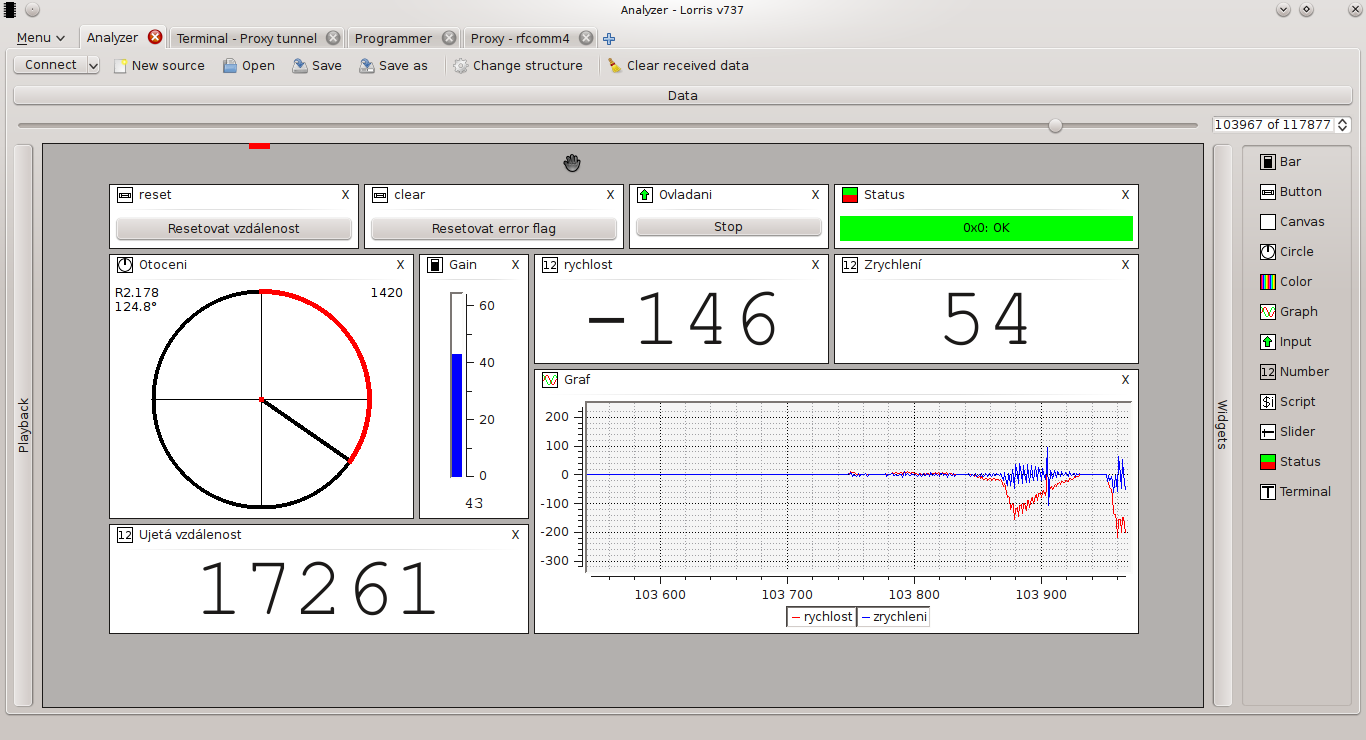
\includegraphics[width=\textwidth]{img/analyzer_all.png}
\caption{Modul analyzér}
\label{Analyzer}
\end{center}
\end{figure}

Tento modul parsuje data (strukturované do packetů) přicházející ze zařízení a zobrazuje je v grafických "widgetech". Zpracovaná data si aplikace ukládá do paměti -- listování packety je možné pomocí posuvníku a boxu v horní části okna. Data (přijatá data, struktura packetů a rozestavení a nastavení widgetů) je také možné uložit do souboru a později zase v programu otevřít.  
\\   
Struktura dat se nastavuje v samostatném dialogu (viz obrázek 3), kde je možno nastavit délku packetu, jeho endianess\cite{endian}, přitomnost hlavičky a její obsah -- statická data ("start byte"), délka packetu(pokud je proměnná), příkaz a ID zařízení. Podle příkazu a ID zařízení je možno později data filtrovat.


\newpage
\setlength{\voffset}{0mm} % posune text/obrázek na této stránce, kam patøí
\pagestyle{plain}

Po nastavení struktury se přijatá data začnou po packetech zobrazovat v horní části okna, a v pravé části se zobrazí sloupeček s dostupnými zobrazovacími widgety. Widgety se dají pomocí drag\&drop principu \uv{vytahat} na plochu v prostřední části okna. Data se k widgetu přiřadí taktéž pomocí drag\&drop, tentokrát přetažení prvního bytu dat na widget. 

Poté widget zobrazuje data tohoto bytu, nebo tento byte bere jako první, pokud jsou data delší. Aby bylo možné zpětně poznat, který byte je k widgetu přiřazen, je po najetí myši na widget červeně zvýrazněn.

Nastavení widgetu jsou přistupná v kontextovém menu po pravém kliknutí myší na widget. Nastavit lze jméno a další parametry podle typu widgetu -- podrobněji jsou možnosti nastavení popsány u jednotlivých widgetů. Widgety je taktéž možné \uv{uzamknout}, aby nebylo možné je zavřít, měnit jejich pozici a velikost.
%(jeho jméno, u čísla např. jeho datový typ apod. - podrobněji jsou možnosti nastavení popsány  u jednotlivých widgetů)

\begin{figure}[h]
\begin{center}
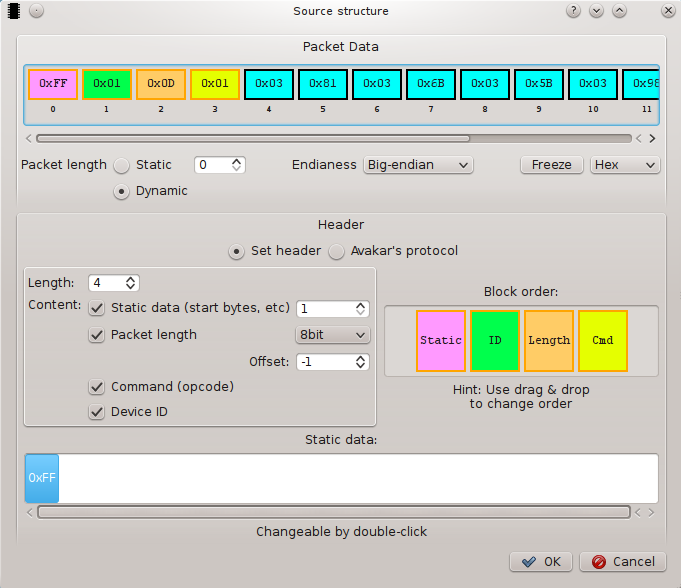
\includegraphics[scale=0.7]{img/analyzer_struct.png}
\caption{Dialog nastavení struktury dat}
\label{Analyzer_struct}
\end{center}
\end{figure}

\begin{figure}[H]
\begin{center}
\subfloat[Seznam widgetů]{\label{analyzer_widgets}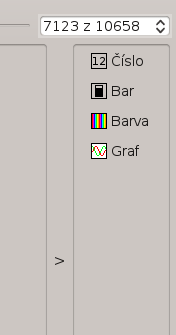
\includegraphics[scale=1]{img/analyzer_widgets.png}}
\hfill
\subfloat[Přiřazení dat pomocí drag\&drop]{\label{analyzer_widgets}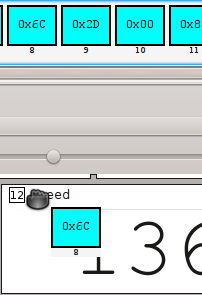
\includegraphics[scale=1]{img/analyzer_drag_data.png}}  
\caption{Widgety}
\label{widgets}
\end{center}
\end{figure}

\subsection*{Widget: číslo}
\addcontentsline{toc}{subsection}{Widget: číslo}
\begin{figure}[h]
\begin{center}
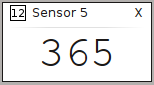
\includegraphics{img/w_num.png}
\end{center}
\end{figure}
Dokáže zobrazovat celá čísla (se znaménkem i bez, 8 až 64 bitů dlouhé) a desetinná čisla (single-precision\footnote{Standartní formát uložení desetinných čísel v jazyku C a dalších (standart IEEE 754-2008).}, 32bit a 64bit).\\
Widget dokáže zarovnat číslo na maximální délku jeho datového typu\\a~formátovat ho těmito způsoby:
\begin{itemize}
    \item Desítkový -- číslo v desítkové soustavě
    \item Desítkový s exponentem -- použije exponent pro zapsaní velkých čísel. Dostupné pouze pro desetinná čísla.
    \item Hexadecimální -- výpis v šestnáctkové soustavě. Dostupné pouze pro přirozená čísla. 
    \item Binární -- zobrazí číslo ve dvojkové soustavě.  Dostupné pouze pro přirozená čísla.
\end{itemize}


%\newpage
\subsection*{Widget: sloupcový bar}
\addcontentsline{toc}{subsection}{Widget: sloupcový bar}
\begin{figure}[h]
\begin{center}
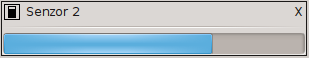
\includegraphics{img/w_bar.png}
\end{center}
\end{figure}
Zobrazuje hodnotu ve sloupcovém baru. Lze nastavit datový typ vstupních dat (stejně jako u čísla), orientaci (vertikální nebo horizontální) a rozmezí zobrazovaných hodnot.

\subsection*{Widget: barva}
\addcontentsline{toc}{subsection}{Widget: barva}
\begin{figure}[h]
\begin{center}
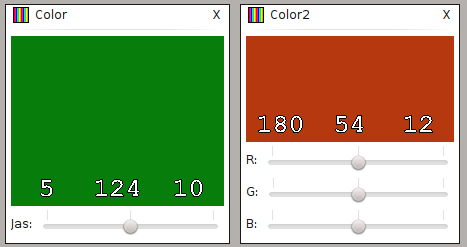
\includegraphics{img/w_col.png}
\end{center}
\end{figure}
Ukáže 24-bitové hodnoty RGB jako barevný obdélník. Dokáže provést korekci jasu všech barev nebo každé z barev RGB zvlášť.

\newpage
\subsection*{Widget: graf}
\addcontentsline{toc}{subsection}{Widget: graf}
\begin{figure}[h]
\begin{center}
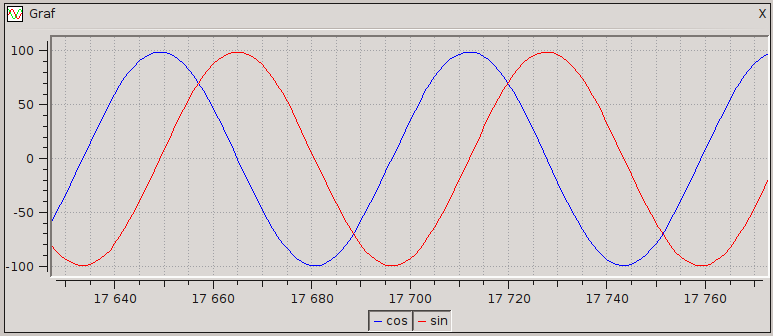
\includegraphics[scale=0.65]{img/w_graph.png}
\end{center}
\end{figure}
Widget graf zobrazuje hodnoty v grafu -- na osu $x$ se vynáší pořadí dat a na osu $y$ hodnoty dat. Lze nastavovat jméno, barvu a datový typ křivky grafu, automatické posouvání grafu, velikost vzorku, měřítko os grafu a zobrazení legendy. Kliknutí na křivku grafu v legendě tuto křivku skryje. Měřítko osy se ovládá otáčením kolečka myši po najetí kurzoru nad osu, po najetí do prostoru grafu se podobně ovládá měřítko celého grafu. 
\begin{figure}[h]
\begin{center}
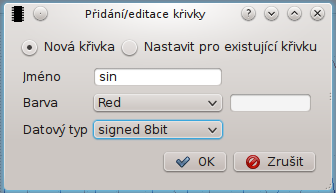
\includegraphics[scale=0.8]{img/w_graph_add.png}
\caption{Dialog pro nastavení parametrů křivky grafu}
\end{center}
\end{figure}

% DOP: přímo ovládání grafu?

\newpage
\subsection*{Widget: script}
\addcontentsline{toc}{subsection}{Widget: script}
\begin{figure}[h]
\begin{center}
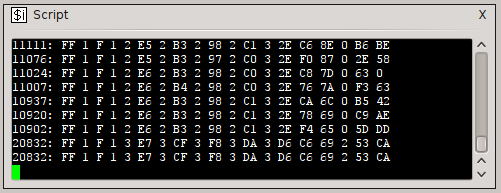
\includegraphics[scale=0.8]{img/w_script.png}
\end{center}
\end{figure}
Tento widget umožňuje zpracovávání dat pomocí scriptu, který si napíše sám uživatel. Jazyk, ve kterém se tento script píše je QtScript\cite{qtscript} (jazyk založený na standartu ECMAScript\cite{ecmascript}, stejně jako JavaScript\cite{javascript}, díky tomu jsou tyto jazyky velmi podobné). Script může zpracovávat příchozí data, reagovat na stisky kláves a posílat data do zařízení. Základní výstup může být zobrazen v terminálu (viz obrázek nad tímto textem), je však možné využít ke zobrazování také ostatní widgety (číslo, bar, ...).
%DOP: že umožní zprcování hodně typů dat?
\begin{figure}[h]
\begin{center}
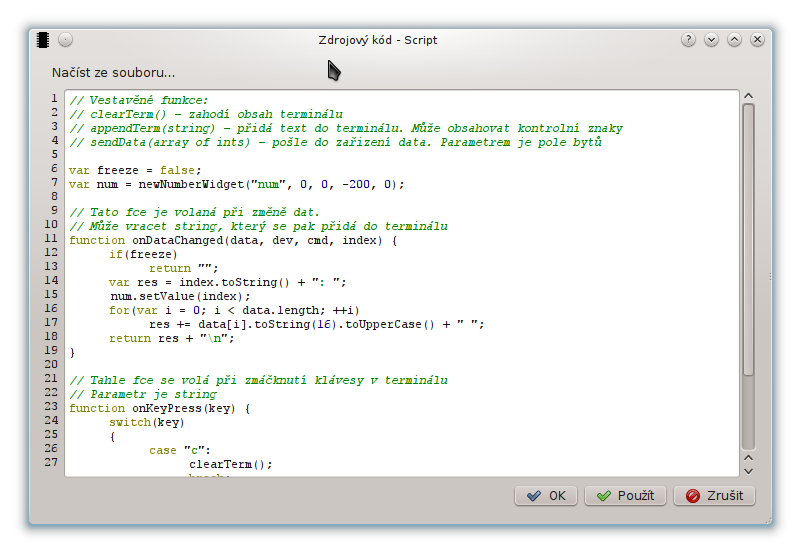
\includegraphics[scale=0.5]{img/w_script_src.png}
\caption{Dialog pro nastavení zdrojového scriptu}
\end{center}
\end{figure}

\newpage
\setlength{\voffset}{0mm} % posune text/obrázek na této stránce, kam patøí
\pagestyle{plain}

\section*{Modul: Proxy mezi sériovým portem a TCP socketem}
\addcontentsline{toc}{section}{Modul: Proxy mezi sériovým portem a TCP socketem} 
\addcontentsline{toc}{subsection}{Popis}

\begin{figure}[h]
\begin{center}
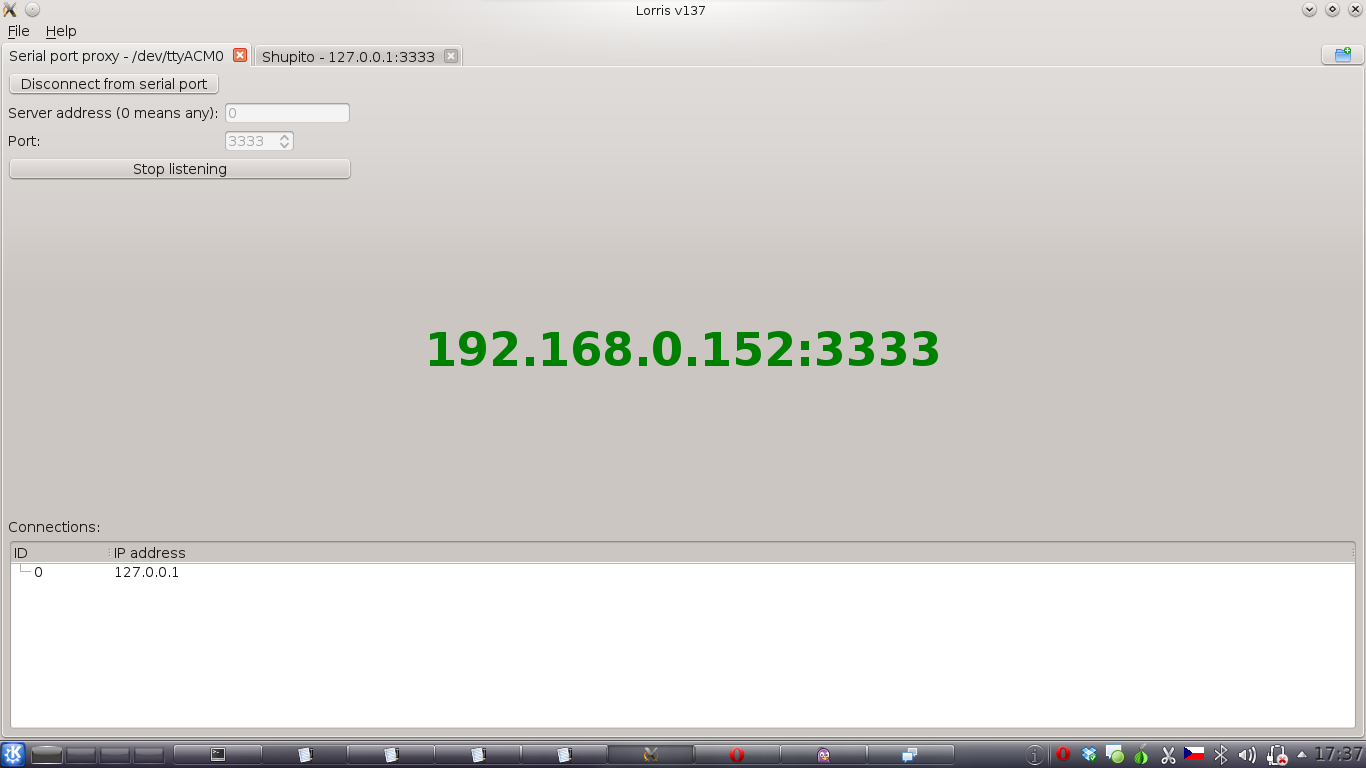
\includegraphics[width=\textwidth]{img/proxy.png}
\caption{Proxy mezi sériovým portem a TCP socketem}
\label{Shupito}
\end{center}
\end{figure}
Jednoduchá proxy mezi sériovým portem a TCP socketem. Vytvoří jednoduchý server, na který je možné se připojit z Lorris nebo jiného programu na jiném počítači. Po připojení se přeposílají data ze sériového portu připojeným klientům a naopak.

\newpage
\setlength{\voffset}{0mm} % posune text/obrázek na této stránce, kam patøí
\pagestyle{plain}

\section*{Modul: Shupito}
\addcontentsline{toc}{section}{Modul: Shupito} 
\addcontentsline{toc}{subsection}{Popis}

\begin{figure}[h]
\begin{center}
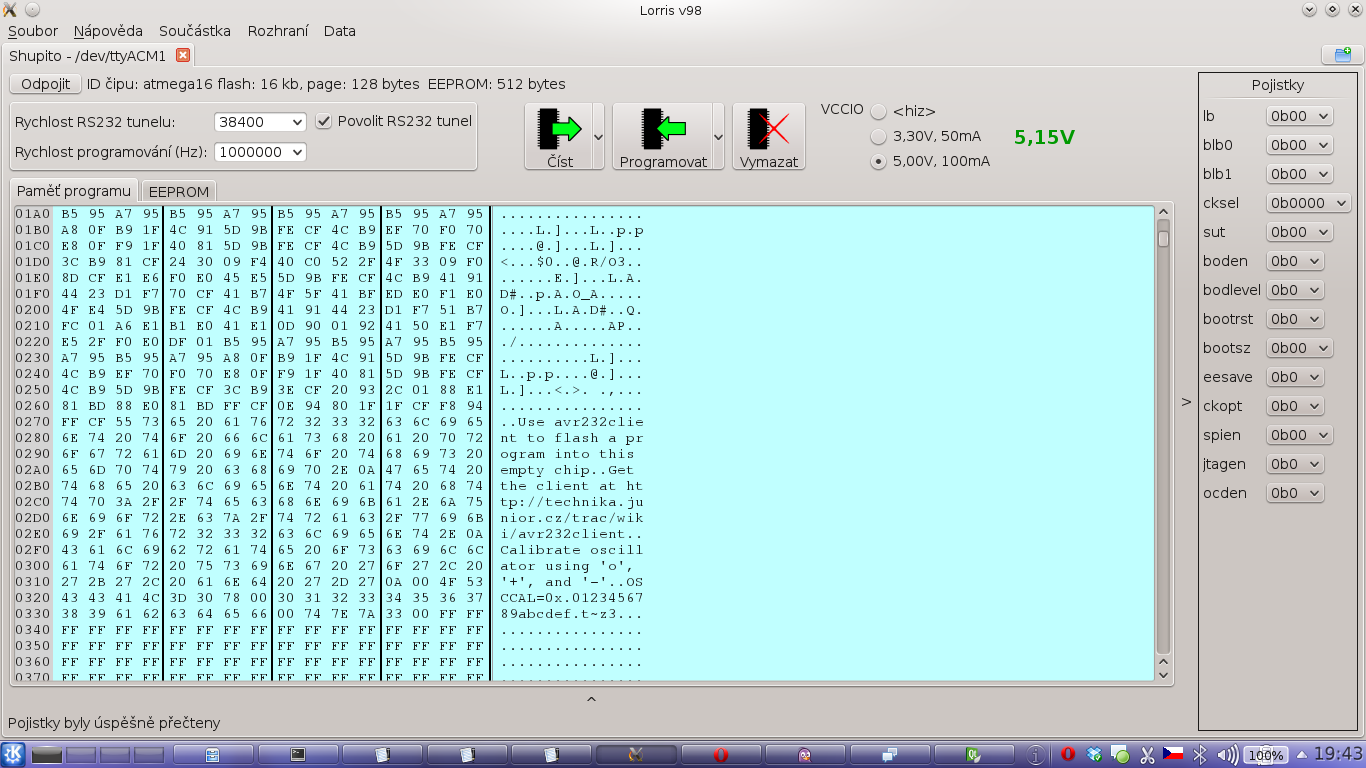
\includegraphics[width=\textwidth]{img/shupito.png}
\caption{Modul Shupito}
\label{Shupito}
\end{center}
\end{figure}
% DOP: popsat typy programováni
Shupito je programátor mikročipů vytvořený Martinem Vejnárem, který dokáže programovat mikrokontroléry pomocí ISP\footnote{\It{In-system programming} -- rozhraní, které umožňuje programovat čipy bez dalšího zařízení přímo v desce plošného spoje.}, PDI a JTAG rozhraní. 

% DOP: opravit
Modul v mojí práci dokáže obsluhovat programátor Shupito -- nastavovat výstupní napětí, číst a programovat paměť čipů (flash i EEPROM) a číst a měnit pojistky. Jako výstupní i vstupní data používá soubory ve formátu Intel HEX32\cite{hex}. 
Způsob komunikace s programátorem je přenesen z oficiálního ovládacího programu\cite{avr232client}, který je však na rozdíl od Lorris dostupný pouze pro MS Windows.

\subsection*{RS232 tunel}
\addcontentsline{toc}{subsection}{RS232 tunel}
\label{tunel}
Shupito dokáže vytvořit tunel\footnote{Přímé spojení programovaného čipu a počítače přes programátor.} pro RS232 linku z programovaného čipu do počítače. Lorris umí této funkce využít -- aktivní tunel se zobrazí jako další typ připojení a je možné se na něj připojit v ostatních modulech.

\newpage
\setlength{\voffset}{0mm} % posune text/obrázek na této stránce, kam patøí
\pagestyle{plain}

\section*{Modul: Terminál}
\addcontentsline{toc}{section}{Modul: Terminál} 
\addcontentsline{toc}{subsection}{Popis}

\begin{figure}[h]
\begin{center}
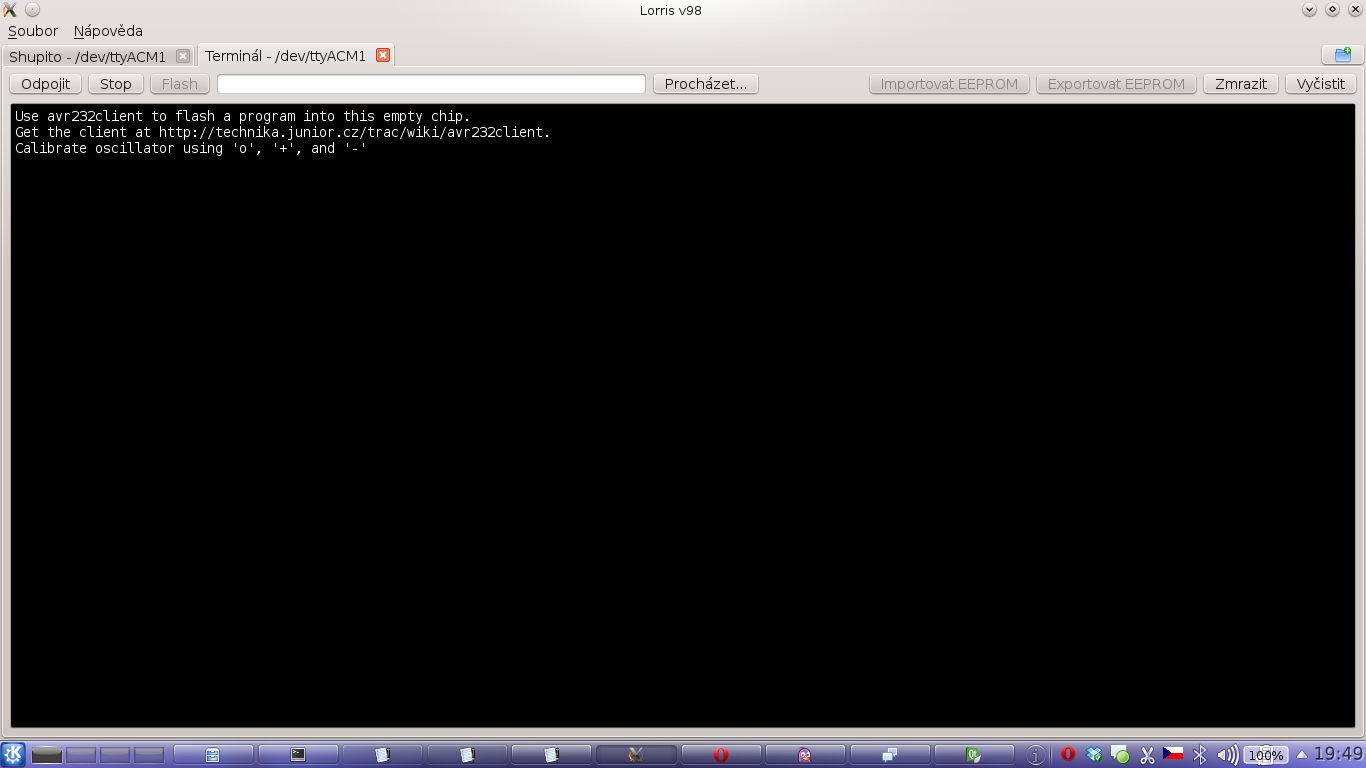
\includegraphics[width=\textwidth]{img/terminal.png}
\caption{Modul terminál}
\label{Terminal}
\end{center}
\end{figure}

Klasický terminál -- zobrazuje data přijatá přes sériový port a posílá stisky kláves. Je obohacený o podporu bootloaderu pro mikrokontroléry AVR ATmega(bootloader byl taktéž napsaný Martinem Vejnarem), který umožňuje jejich programování přes RS232 linku. Informace o protokolu bootloaderu jsem získal z oficiálního programu určeného k programování přes tento\\bootloader, avr232client\cite{avr232client}.


\newpage
\section*{Příklady použití}
\addcontentsline{toc}{section}{Příklady použití}
\subsection*{1. Testování barevného senzoru}
\addcontentsline{toc}{subsection}{1. Testování barevného senzoru}
{\bf Situace:} Stavím robota do soutěže (Eurobot, RobotChallange, ...), ve které je možné se na herním poli orientovat podle barvy. Chci barevný senzor otestovat, proto jsem na nepájivém poli postavil jednoduchý obvod s čipem, na který je senzor připojený. Čip bude dávat senzoru pokyny k měření a vyčítat z něj RGB hodnoty, které následně pošle do RS232 linky.\\
\\
{\bf Řešení:} Program, který bude ze senzoru číst hodnoty naprogramuji do čipu pomocí programátoru Shupito, který také poskytne tunel pro RS232 linku. Na tento tunel se připojím modulem Analyzér, ve kterém díky widgetu "barva" mohu vidět barvu, kterou senzor rozpoznal.

\begin{figure}[h]
\begin{center}
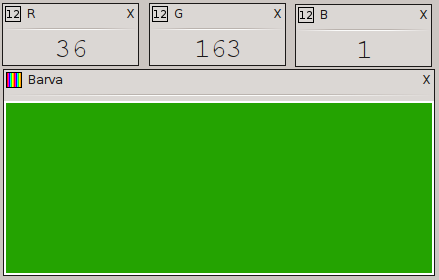
\includegraphics{img/use_color.png}
\caption{Barva v modulu Analyzér}
\label{Terminal}
\end{center}
\end{figure}

\newpage
\subsection*{2. Testování enkodérů}
\addcontentsline{toc}{subsection}{2. Testování enkodérů}
{\bf Situace:} Potřebuji otestovat přesnost magnetických enkodérů, které však odesílají data o úhlu natočení rozdělené v několika bytech v takovém formátu, který znemožňuje použití např. terminálu.\\
\\
{\bf Řešení:} Nechci za tímto účelem stavět a programovat novou desku s dalším mikročipem, připojím tedy enkodér k počítači. V Lorris otevřu modul analyzér a ve widgetu "script" napíšu jednochý script, který složí úhel do jednoho čísla a zobrazí ho ve widgetu "číslo".

% DOP: screenshot

\newpage
\subsection*{3. Ladění PID regulátoru}
\addcontentsline{toc}{subsection}{3. Ladění PID regulátoru}
{\bf Situace:} Robot kvůli rozdílnému výkonu motorů nejede rovně. Tento problém jsem se rozhodl řešit pomocí PID regulátoru, pro jehož správnou funkci je potřeba nastavit několik konstant. \\
\\
{\bf Řešení:} Program v robotovi mi posílá aktualní výkon motorů a nastavení konstant PID regulátoru a umožňuje přenastavení těchto konstant a ovládání robota. Tento program do robota nahrávám přes bluetooth pomocí modulu Terminál, protože čip má v sobě bootloader -- díky tomu nemusím mít připojený programátor.  

V modulu analyzér si zobrazím aktuální hodnoty PID regulátoru (jako číslo) a výkon motorů (jako graf či číslo). Do widgetu script napíšu jednoduchý script, který po stisku kláves změní nastavení konstant regulátoru nebo rozjede/zastaví robota.

\newpage
\setlength{\voffset}{0mm} % posune text/obrázek na této stránce, kam patøí
\pagestyle{plain}

\section*{Knihovny třetích stran, licence}
\addcontentsline{toc}{section}{Knihovny třetích stran, licence}
\subsection*{Knihovny třetích stran}
\addcontentsline{toc}{subsection}{Knihovny třetích stran}
{\bf Qwt}\cite{qwt_link} je knihovna pro Qt Framework obsahující tzv. widgety pro aplikace technického charakteru -- grafy, sloucové ukazatele, kompasy a podobně. Ve svojí práci
zatím z této knihovny používám pouze graf (v modulu analyzéru). \\
{\bf QExtSerialPort}\cite{qext_link} poskytuje připojení k sériovému portu a také dokáže vypsat seznam nalezených portů v počítačí.\\
{\bf QHexEdit2}\cite{qhex_link} je hex editor použitý v modulu programátoru Shupito na zobrazování obsahu paměti. V této knihovně jsem upravoval několik málo drobností, 
týkajících se především vzhledu.

\subsection*{Licence}
\addcontentsline{toc}{subsection}{Licence}
Lorris je dostupný pod licencí GNU GPLv3, licence použitých programů a knihoven jsou následující:
\begin{itemize}
    \item {\bf Qt Framework} je distribuován pod licencí GNU LGPLv2.1
    \item {\bf Qwt} je distribuováno pod Qwt license, která je založená na GNU LGPLv2.1
    \item {\bf QExtSerialPort} je distribuován pod The New BSD License
    \item {\bf QHexEdit2} je distribuován pod licencí GNU LGPLv2.1
    \item {\bf avr232client} je distribuován pod licencí Boost Software License v1.0
\end{itemize}

%%%%%%%%%%%%%%%%%%%%%%%%%%%%%%%%%%%%%%%%%%%%%%%%%%%%%%%%%%%%%%%%%%%%%%%%%%%
\newpage
\addcontentsline{toc}{section}{Reference}
 \begin{thebibliography}{99}
 %% 99 znamená, že maximální délka čísla literatury jsou dva znaky
% seznam samozřejmě změníte podle svého, tohle je pouze ukázka formátování
    \bibitem{qtfw} \It{Qt Framework -- Cross-platform application and UI framework} \\
    \url{http://qt.nokia.com/} (Stav ke dni 28.1.2012)

    \bibitem{tcp_sock} \It{TCP socket} \\
    \url{http://en.wikipedia.org/wiki/Transmission_Control_Protocol} (Stav ke dni 25.2.2012)

    \bibitem{repo} \It{GIT repozitář Lorris} \\
    \url{https://github.com/Tasssadar/Lorris}

    \bibitem{qwt_link} \It{Qt Widgets for Technical Applications} \\
    \url{http://qwt.sourceforge.net/} (Stav ke dni 22.2.2012)

    \bibitem{qext_link} \It{Qt interface class for old fashioned serial ports} \\
    \url{http://code.google.com/p/qextserialport/} \\
    (Stav ke dni 22.2.2012)

    \bibitem{qhex_link} \It{Binary Editor for Qt} \\
    \url{http://code.google.com/p/qhexedit2/} (Stav ke dni 22.2.2012)
    
    \bibitem{shupito} \It{Shupito -- Programátor} \\
    \url{http://shupito.net/} (Stav ke dni 28.1.2012)

    \bibitem{avr232client} \It{avr232client} \\
    \url{http://technika.junior.cz/trac/wiki/avr232client}\\
    (Stav ke dni 28.1.2012)

    \bibitem{endian} \It{Endianness} \\
    \url{http://en.wikipedia.org/wiki/Endianness} (Stav ke dni 28.1.2012)

    \bibitem{qtscript} \It{QtScript -- Making Applications Scriptable} \\
    \url{http://developer.qt.nokia.com/doc/qt-4.8/scripting.html} (Stav ke dni 26.2.2012)

    \bibitem{ecmascript} \It{ECMAScript} \\
    \url{http://en.wikipedia.org/wiki/ECMAScript} (Stav ke dni 26.2.2012)

    \bibitem{javascript} \It{JavaScript} \\
    \url{http://en.wikipedia.org/wiki/JavaScript} (Stav ke dni 26.2.2012)

    \bibitem{float} \It{Single-precision floating-point format} \\
    \url{http://en.wikipedia.org/wiki/Single_precision} (Stav ke dni 28.1.2012)

    \bibitem{hex} \It{Intel HEX} \\
    \url{http://en.wikipedia.org/wiki/Intel_hex} (Stav ke dni 28.1.2012)
\end{thebibliography}

\end{document}